\documentclass[tikz,border=2pt]{standalone}
\usepackage{amsmath}
\usetikzlibrary{arrows.meta}
\begin{document}
% One (s,S) cycle, Lighthouse case s = 16, S = 20, demands 2, 1, 4: positions 20, 18, 17 pay the
% running costs L(20) = 10.3, L(18) = 8.97, L(17) = 8.3 (L(x) = (2/3)(x - 4.55) for x >= 10);
% the end-of-period position 13 <= s enters the hitting set and the hitting cost K = 50 is paid.
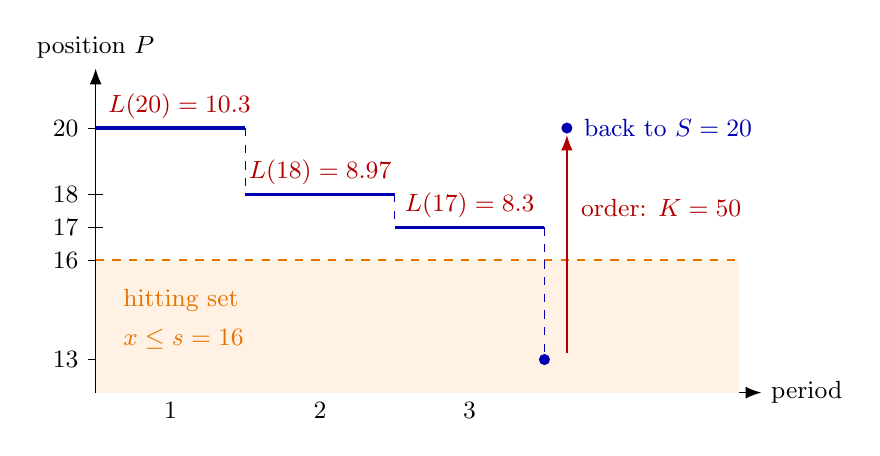
\begin{tikzpicture}[font=\small, >={Latex[length=2mm]}, x=1.9cm, y=0.42cm]
  % axes
  \draw[->] (0,12) -- (4.45,12) node[right] {period};
  \draw[->] (0,12) -- (0,21.8) node[above] {position $P$};
  \foreach \y in {13,16,17,18,20} \draw (0.05,\y) -- (-0.05,\y) node[left] {$\y$};
  \foreach \k in {1,2,3} \node[below] at (\k-0.5,12) {$\k$};
  % hitting set
  \fill[orange!10] (0,12) rectangle (4.3,16);
  \draw[orange!90!black, thick, dashed] (0,16) -- (4.3,16);
  \node[orange!90!black, anchor=west] at (0.12,14.8) {hitting set};
  \node[orange!90!black, anchor=west] at (0.12,13.6) {$x\leq s=16$};
  % path of the position
  \draw[blue!70!black, very thick] (0,20) -- (1,20);
  \draw[blue!70!black, very thick] (1,18) -- (2,18);
  \draw[blue!70!black, very thick] (2,17) -- (3,17);
  \draw[blue!70!black, thin, dashed] (1,20) -- (1,18) (2,18) -- (2,17) (3,17) -- (3,13);
  \fill[blue!70!black] (3,13) circle (2pt);
  % running costs
  \node[red!70!black, anchor=south] at (0.56,20) {$L(20)=10.3$};
  \node[red!70!black, anchor=south] at (1.5,18) {$L(18)=8.97$};
  \node[red!70!black, anchor=south] at (2.5,17) {$L(17)=8.3$};
  % order back to S
  \draw[->, red!70!black, thick] (3.15,13.2) -- (3.15,19.8);
  \node[red!70!black, anchor=west] at (3.18,17.6) {order: $K=50$};
  \fill[blue!70!black] (3.15,20) circle (2pt);
  \node[blue!70!black, anchor=west] at (3.2,20) {back to $S=20$};
\end{tikzpicture}
\end{document}
